\documentclass{article}
\usepackage[utf8]{inputenc}
\usepackage{listings}
\usepackage{graphicx}
\usepackage{tcolorbox}
\graphicspath{{./}}
\title{
	Report Iot Interfaces From Hardware To 			Software And Wireless Communication
		\\[1\baselineskip]
	Subject: TP Capteurs et environment, 2021
}
\author{
	Author: Duc Dinh Anh
        \\[1\baselineskip]
	Email: ducda.m20ict@st.usth.edu.vn
        \\[1\baselineskip]
	Mobile: (+84) 982 086 651
}
\date{July 2021}

\lstdefinestyle{mystyle}{
    basicstyle=\small,   
    tabsize=2,
    autogobble=true
}
\lstset{style=mystyle}

\maketitle
\newpage
\begin{document}
\section{Compute geographic bounding box}
\subsection{*What is geographic bounding box ?}
\raggedright

	- \textbf{Bounding box} is the limitation or the border which contains all the sensor of our system, according to my knowledge bounding box is also the perfect area in which the sensor can interact efficiently. Beside, bounding box can determine the distance of the sensors and how far the signal can reach.

\\[1\baselineskip]
\centering{\begin{pic1}}
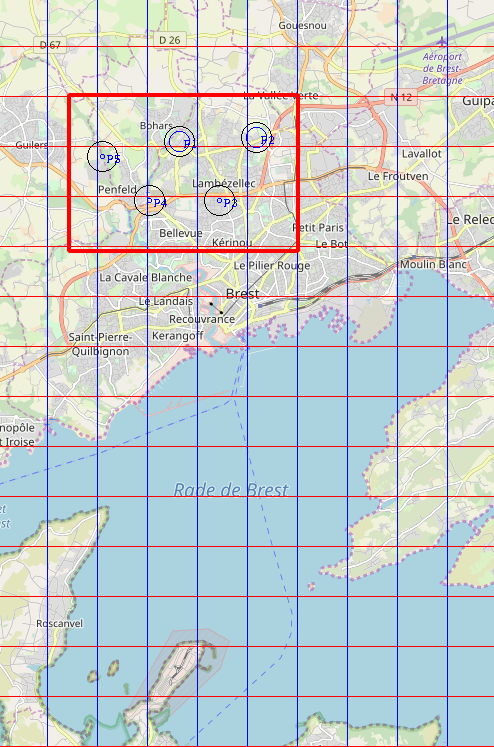
\includegraphics[width=0.80\textwidth]{iot_project}
\\
\caption{Figure 1: The red bounder is the bounding box in physical world.}
\end{pic1}
\\[1\baselineskip]
\raggedright
\subsection{*How can we determine the bounding box ?}

- \textbf{Step 1}: We need to create the behaviour file whose name is "nodes-test-include.occ". In this file, we need to add two processes one is "Node" and the other is "Mux". "Node" represents the sensor, "Mux" is the process that displays all the output from "Node".

\\[2\baselineskip]

- \textbf{Step 2}: We need to get the x-y coordinator of each sensor by using the "Node" process in "nodes-test-include.occ" file. To do that we can access to the global array "NetLocation" in "halongtpnet.occ" file which contains all the information of each sensor.

\\[2\baselineskip]

- \textbf{Step 3}: After we find the bounding box, we need to use cooperation techniques to send the coordinator of bounding box to all sensor.

\\[2\baselineskip]

- \textbf{*Note}: To find the bounding box we need to find the most left and most right value of the coordinator.

\\[1\baselineskip]

\subsection{Code}
\begin{tcolorbox}
\begin{lstlisting}
DATA TYPE BBox
  RECORD
    INT Top,Left,Bottom,Right:
:
PROTOCOL diam.proto IS BBox: -- Output type is BBox 
PROC Node([]CHAN OF diam.proto in,out, VAL INT Identity,
CHAN OF BYTE toMux)
  -- MyXLoc, MyYLoc are variables which store xLoc, yLoc
  INT MyXLoc:
  INT MyYLoc:
  -- 
  [MaxFanOut] BBox BBuf:
  BBox myBBox:
  SEQ
    MyXLoc := NetLocation[Identity][xLoc]
    MyYLoc := NetLocation[Identity][yLoc]
    -- Initial BBOX
    myBBox[Left] := MyXLoc
    myBBox[Right] := MyXLoc
    myBBox[Top] := MyYLoc
    myBBox[Bottom] := MyYLoc
\end{lstlisting}
\end{tcolorbox}
\begin{tcolorbox}
\begin{lstlisting}
    SEQ Turns=0 FOR MaxNodes-1
      SEQ
      -- Create input and ouput section
        PAR
          PAR i=0 FOR SIZE out
            out[i] ! myBBox
          PAR i=0 FOR SIZE in
            in[i] ? BBuf[i]
        -- Calculate max left, right, top, bottom section
        SEQ i=0 FOR SIZE in
          SEQ
            IF
              myBBox[Left] > BBuf[i][Left]
                myBBox[Left] := BBuf[i][Left]
              TRUE
                SKIP
            IF
              myBBox[Right] > BBuf[i][Right]
                myBBox[Right] := BBuf[i][Right]
              TRUE
                SKIP
            IF
              myBBox[Top] > BBuf[i][Top]
                myBBox[Top] := BBuf[i][Top]
              TRUE
                SKIP
            IF
              myBBox[Bottom] > BBuf[i][Bottom]
                myBBox[Bottom] := BBuf[i][Bottom]
              TRUE
                SKIP
    -- Printing section
    toMux ! 'L'
    toMux ! ':'
    out.number(myBBox[Left], 0, toMux)
    toMux ! ' '
    toMux ! 'R'
    toMux ! ':'
    out.number(myBBox[Right], 0, toMux)
    toMux ! ' '
    toMux ! 'T'
    toMux ! ':'
    out.number(myBBox[Top], 0, toMux)
    toMux ! ' '
    toMux ! 'B'
    toMux ! ':'
    out.number(myBBox[Bottom], 0, toMux)
    toMux ! '*n'
    SKIP
:
\end{lstlisting}
\end{tcolorbox}
\newpage
\subsection{Result}
\\[2\baselineskip]
\begin{tcolorbox}
Compile command: Kroc -lcourse halongtpnet.occ 
\end{tcolorbox}
\\[2\baselineskip]
\begin{tcolorbox}
Run command: ./halongtpnet
\end{tcolorbox}
\\[2\baselineskip]
\centering{\begin{pic2}}
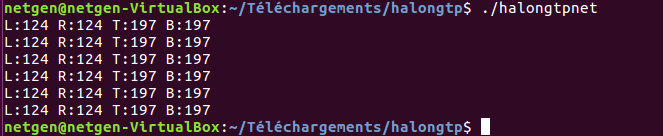
\includegraphics[width=0.80\textwidth]{iot_project_2}
\\
\caption{Figure 2: Display bounding box coordinator on terminal.}
\end{pic2}
\raggedright
\section{Find the maximum elevation}
\raggedright
\subsection{*How can we find the elevation of each cell ?}

- \textbf{Step 1}: We need to create the behaviour file whose name is "nodes-test-include-cell.occ". In this file, we need to add two processes one is "CellNode" and the other is "Mux". "CellNode" represents each cell in the map, "Mux" is the process that displays all the output from "CellNode".

\\[2\baselineskip]

- \textbf{Step 2}: We need to get the elevation of each sensor by using the "CellNode" process in "nodes-test-include-cell.occ" file. First, we can get all the parameter of all cell in the "halongtpData0.occ". Second, through these parameters we can access to each "CellNode" in the "halongtp0.occ" so that we can get the elevation of each cell.

\\[2\baselineskip]

- \textbf{Step 3}: After we find the elevation, we need to use cooperation techniques to send the elevation to all sensor and find the maximum elevation.

\\[2\baselineskip]

\subsection{Code}
\begin{tcolorbox}
\begin{lstlisting}
PROTOCOL diam.proto IS REAL64: -- Output type is REAL64
PROC CellNode([]CHAN OF diam.proto in,out, 
VAL INT Identity, CHAN OF BYTE toMux)
  -- Get all cells in the array
  CellArray myCell: 
  -- Get position of each cell
  CellPosition myPosition:
  -- Get currently elevation
  REAL64 myElevation:
  -- Buffer is used to store all the elevations
  [MaxFanOut] REAL64 elvBuf:
  SEQ
    myCell := Cells[Identity]
    myPosition := myCell[position]
    myElevation := myPosition[elevation]
    SEQ Turns=0 FOR MaxNodes-1
      SEQ
        PAR
          PAR i=0 FOR SIZE in
            in[i] ? elvBuf[i]
          PAR i=0 FOR SIZE out
            out[i] ! myElevation
        SEQ i=0 FOR SIZE in
           IF 
            elvBuf[i] > 0.0 -- Elevation <= 0 is sea
              IF     -- Keep updating until find sea  
                myElevation < elvBuf[i]
                  myElevation := elvBuf[i]
                TRUE
                  SKIP
            TRUE
              SKIP
    out.real64(myElevation, 0, 0, toMux)
    toMux ! '*n'
:
\end{lstlisting}
\end{tcolorbox}
\newpage
\subsection{Result}
\\[2\baselineskip]
\begin{tcolorbox}
Compile command: Kroc -lcourse halongtp0.occ 
\end{tcolorbox}
\\[2\baselineskip]
\begin{tcolorbox}
Run command: ./halongtp0 
\end{tcolorbox}
\\[2\baselineskip]
\centering{\begin{pic3}}
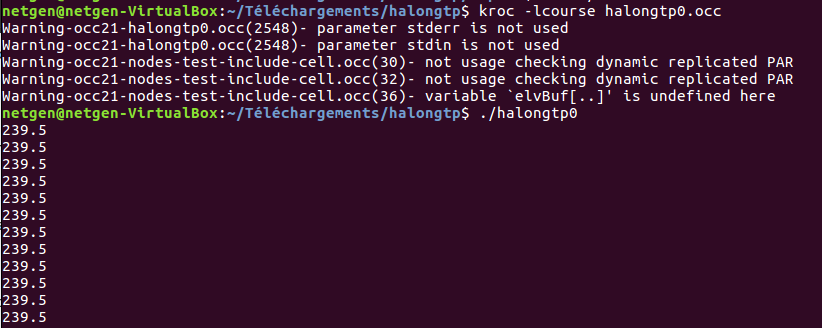
\includegraphics[width=0.80\textwidth]{iot_project_3}
\\
\caption{Figure 3: Display maximum elevation on terminal.}
\end{pic3}

\newpage
\raggedright
\subsection{Generate "*.ppm" files, convert to "*.mp4" file}
\begin{tcolorbox}
\begin{lstlisting}
etc................

#USE "course.lib"

VAL INT MaxFanOut IS 4:

VAL INT MaxNodes IS 837:

-- Uncomment to test generate PPM feature
--#INCLUDE "./testGeneratePPM/nodes-test-include-cell-ver2.occ" -- Gen ppm

-- Uncomment to Calculate max elevation
#INCLUDE "nodes-test-include-cell.occ" -- Caculate max elevation
PROC halongtp0(CHAN OF BYTE stdin, stdout, stderr)

................etc
\end{lstlisting}
\end{tcolorbox}
\\[1\baselineskip]

- \textbf{*Note:} To use this feature. 

\\[1\baselineskip]

- \textbf{First}, we need to Find the section above in "halongtp0.occ" file. 

\\[1\baselineskip]

- \textbf{Second}, uncomment the line below:

\\[1\baselineskip]

\textbf{#INCLUDE "./testGeneratePPM/nodes-test-include-cell-ver2.occ"}
 
\\[1\baselineskip]

- \textbf{Last}, comment the line below: 

\\[1\baselineskip]

\textbf{#INCLUDE "nodes-test-include-cell.occ"}.

\\[1\baselineskip]
\begin{tcolorbox}
Compile command: make cinema/ sudo make cinema 
\end{tcolorbox}
\\[1\baselineskip]
\begin{tcolorbox}
Clean *.ppm files command: make clean
\end{tcolorbox}
\end{document}

